\documentclass[11pt]{scrartcl}
\usepackage{graphicx}
\graphicspath{{./}}
\usepackage[sexy]{evan}
\usepackage[normalem]{ulem}
\usepackage{hyperref}
\usepackage{mathtools}
\hypersetup{
    colorlinks=true,
    linkcolor=blue,
    filecolor=magenta,      
    urlcolor=cyan,
    pdfpagemode=FullScreen,
    }
\usepackage[most]{tcolorbox}
\renewcommand{\dangle}{\measuredangle}

\renewcommand{\baselinestretch}{1.5}

\addtolength{\oddsidemargin}{-0.4in}
\addtolength{\evensidemargin}{-0.4in}
\addtolength{\textwidth}{0.8in}
% \addtolength{\topmargin}{-0.2in}
% \addtolength{\textheight}{1in} 


\setlength{\parindent}{0pt}

\usepackage{pgfplots}
\pgfplotsset{compat=1.15}
\usepackage{mathrsfs}
\usetikzlibrary{arrows}

\title{Problem Set 1}
\author{Azzam Labib (IG: haxuv.world)}
\date{G5-6| Sat, 22 June 2024}
\begin{document}
\maketitle

\begin{enumerate}
    \item Find the sum of all the 1-digit prime factors of 13262613.

    \item Bind 4 straws which are 4cm in diameter with a $a+b\pi$ cm long string. If both $a$ and $b$ are integers, find $a \times b$. (The knot does not take into consideration.)

    \item Given 4 different positive integers $a$, $b$, $c$, and $d$ that satisfy $\frac{1}{a} + \frac{1}{b} + \frac{1}{c} + \frac{1}{d} = 1$. Find the minimum value of $a+b+c+d$.

    \item Given that the digits of a 4-digit number $A$ are even numbers, the digits of a 4-digit number $B$ are odd numbers, and the digits of a number $C$ are the alternation of odd and even numbers. If $C = A + B$, find the maximum value of $C$.

    \item In Jumping Grid, the player jumps 1 grid or 2 grids forward each time, such as jump from $\square$ to $\square$ or $\square$. If David is at $\square$, how many ways are there for him to jump to $\square$?
    \begin{figure}[h]
        \centering
        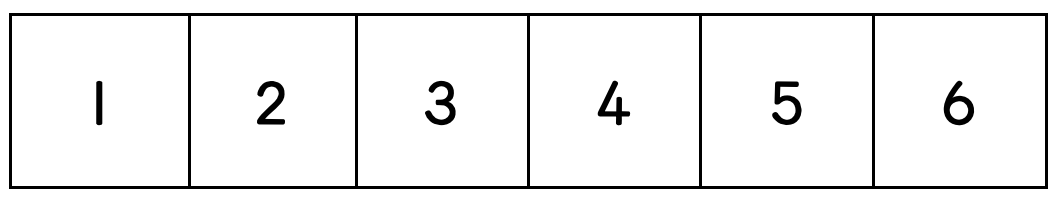
\includegraphics[scale=0.5]{StarGen/0Figure/jumping-grid-wmi-2020-g5-6.png}
    \end{figure}

    \item If $\angle A = 35^\circ$, $\angle B = 40^\circ$, $\angle C = 30^\circ$, find the degrees of $\angle D + \angle E + \angle F$.
    \begin{figure}[h]
        \centering
        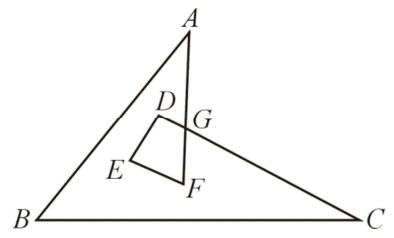
\includegraphics[scale=1.05]{StarGen/0Figure/weird-triangle-wmi-2020-g5-6.png}
    \end{figure}

    \item The result of $123456789 \times 36 \times 5$ has $a$ 0's, $b$ 1's, and $c$ 2's. Find the 3-digit number $\overline{abc}$.

    \item The units digit and the tens digit of a 2-digit number are composite numbers that are coprime. When the 2-digit number has the largest value, how many factors does it have?
    
    \item Cut a cuboid whose surface is painted red into several cubes of 1 cm$^3$. Suppose only 3 cubes don't have any red faces, find the volume of the original cuboid in cm$^3$.
    
    \item As shown, $ABCD$ is a square, $DE$ intersects $CE$ at $E$, $DE$ intersects $AC$ at $F$, $\angle DEC = 24^\circ$. Find $\angle EFB$.
    \begin{figure}[h]
        \centering
        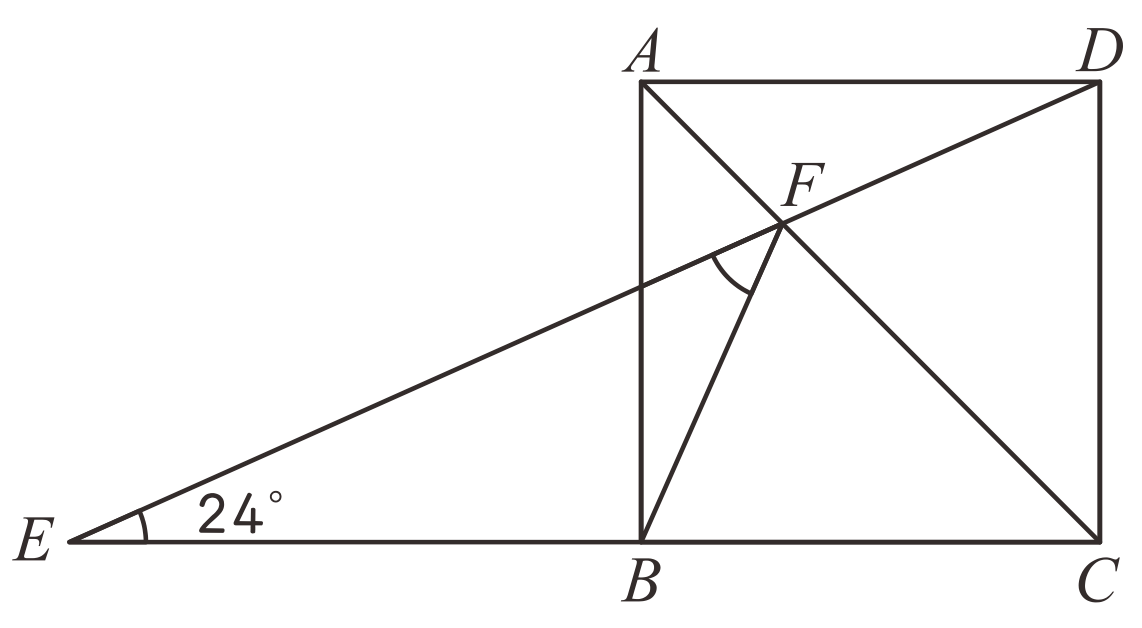
\includegraphics[scale=0.43]{StarGen/0Figure/geometry-wmi-2023-g5.png}
    \end{figure}
    
    \item Insert three bamboo poles A, B, and C in the ground at the depth of $x$ cm. If the parts of the three bamboo poles above the ground are $\frac{2}{3}$, $\frac{3}{4}$, and $\frac{1}{3}$ of each of their total lengths, respectively, find the ratio of the lengths of A, B, and C.
    
    \item Below is the math test result of a class of 41 students. Find the median and mode of their scores.\\
    
    \begin{tabular}{|c|c|c|c|c|c|c|}
    \hline
    Score & 50 & 60 & 70 & 80 & 90 & 100 \\
    \hline
    Number of People & 1 & 12 & 8 & 13 & 4 & 3 \\
    \hline
    \end{tabular}
    
    \item In a train carriage, $\frac{1}{4}$ of the passengers are young people, $\frac{2}{3}$ of the passengers are middle-aged people, and the rest are elderly people. Suppose there are 6 elderly people, and the number of seats in the carriage is $\frac{3}{4}$ of the number of passengers. How many passengers don't have a seat?
    
    \item The sum of three large, medium, and small numbers is 166. Given that the quotients of the large number divided by the medium number and the medium number divided by the small number are both 3, and their remainders are both 2, find the sum of all the digits of the large number.

    
    \item In a bag are 11 balls which are marked 1--11. How many balls should Roy take from the bag the least to make sure that at least two of the numbers on the balls are prime numbers?
    
    \item How many 6-digit numbers $x2023y$ are divisible by 286?
    
    \item Find the sum of all the digits of M.
    \[M = (1 - \frac{1}{2}) \times (2 - \frac{2}{3}) \times (3 - \frac{3}{4}) \times \cdots \times (8 - \frac{8}{9}) \times (9 - \frac{9}{10})\]
    
    \item Pour some water in a semicylinder container so that the angle between the rectangular face of the container and the water surface is $45^\circ$. Find the volume of the water in cm$^3$. ($\pi = 3.14$)
    \begin{figure}[h]
        \centering
        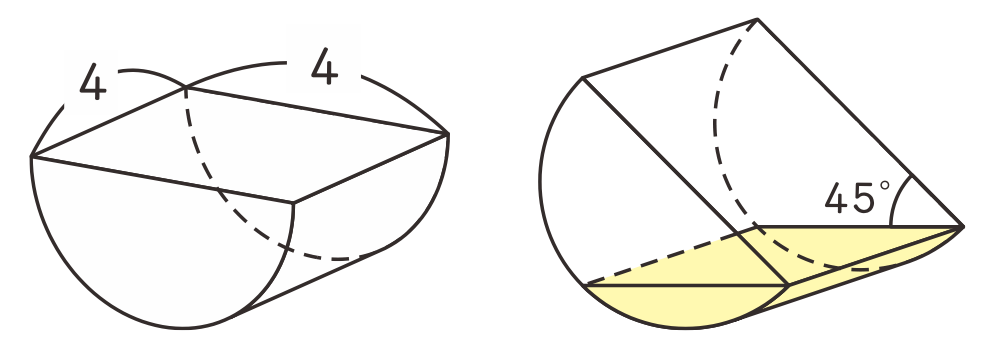
\includegraphics[scale=0.5]{StarGen/0Figure/45-degree-cylinder-wmi-2023-g5.png}
    \end{figure}
    
    \item Draw 3 different diagonals in a regular hexagon at will to make it a line symmetric figure. How many different line symmetric figures can be drawn at most? (If figures look the same after rotation, they are the same one)
    
    \item The last two digits of $1 + 2 + 3 + \cdots + n$ are 03, and its hundreds digit is not 0. If $n$ is no larger than 100, find the sum of all the digits of the smallest $n$.
\end{enumerate}

% Note: For problems 3, 9, and 13, you would need to include the specific diagrams or images to fully represent the questions in LaTeX.

\end{document}